\setcounter{page}{1} % 从下面开始编码
\chapter{安装}
\section{下载镜像} 
\href{https://mirrors.tuna.tsinghua.edu.cn/}{点击访问清华源官网}

% 可以到\href{https://mirrors.tuna.tsinghua.edu.cn/deepin-cd/}{清华源}下载最新的系统镜像

%\begin{figure}[hbt!] 
%	\centering
%	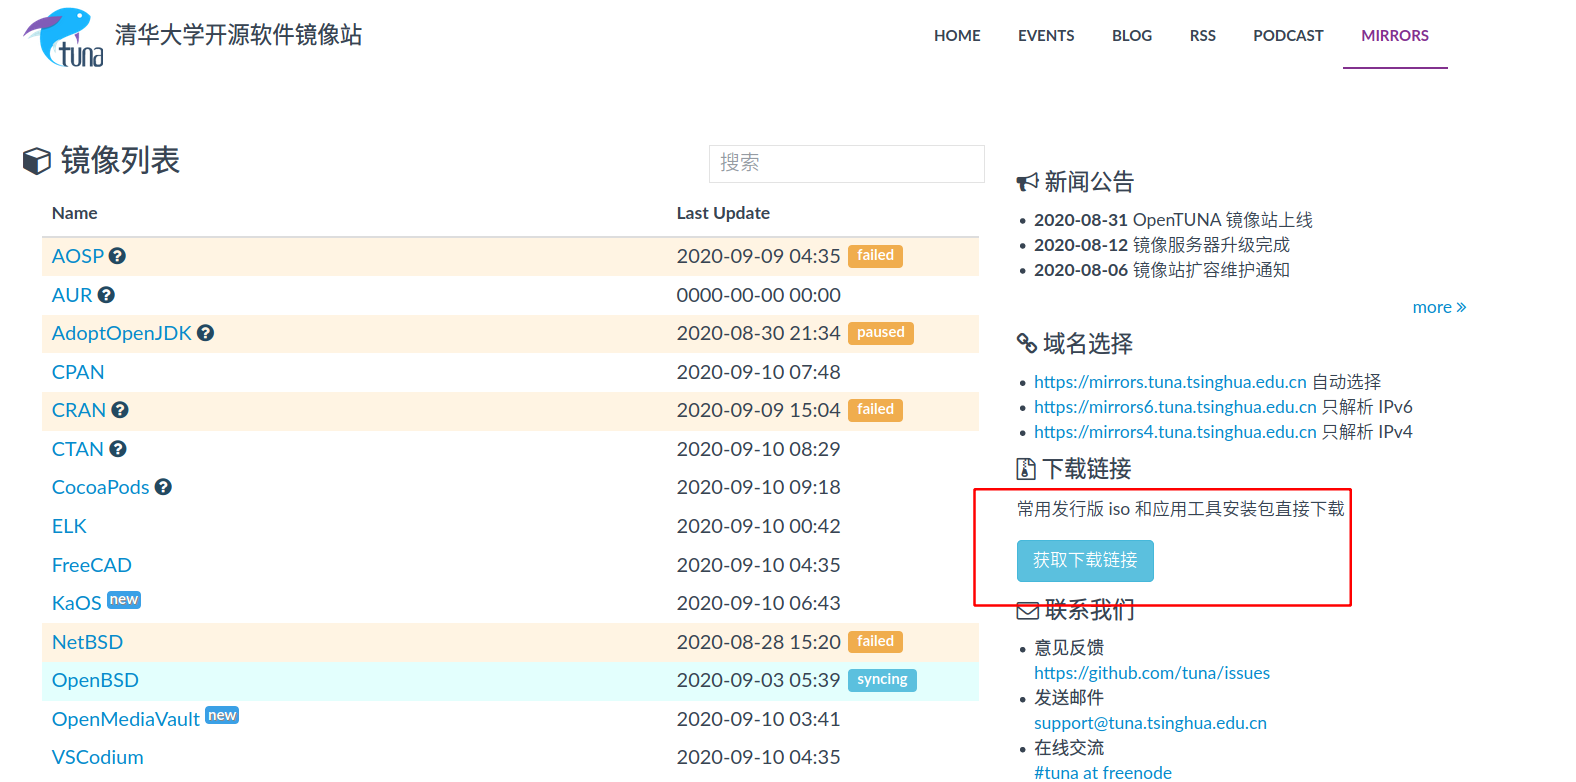
\includegraphics[width=0.49\textwidth]{./img/install/1.png}
%	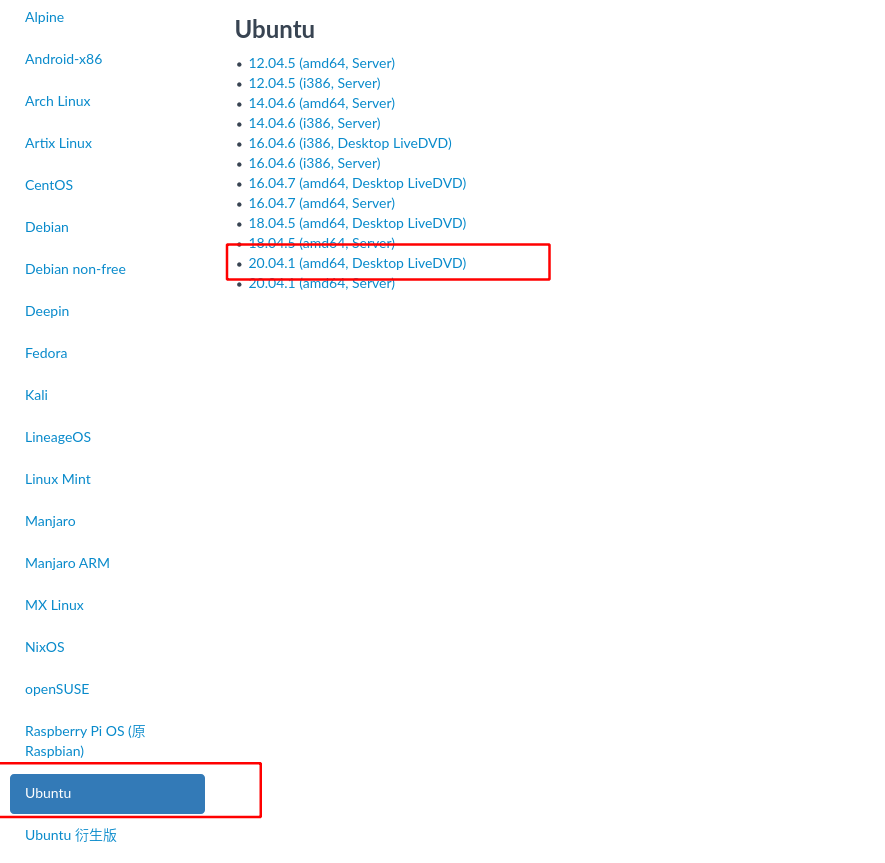
\includegraphics[width=0.49\textwidth]{./img/install/2.png}
%	\caption{镜像下载步骤} %caption是图片的标题
%	\label{fig:ubuntu_download} % 交叉引用
%\end{figure}

\begin{figure}[h!]
	\subfloat[1]{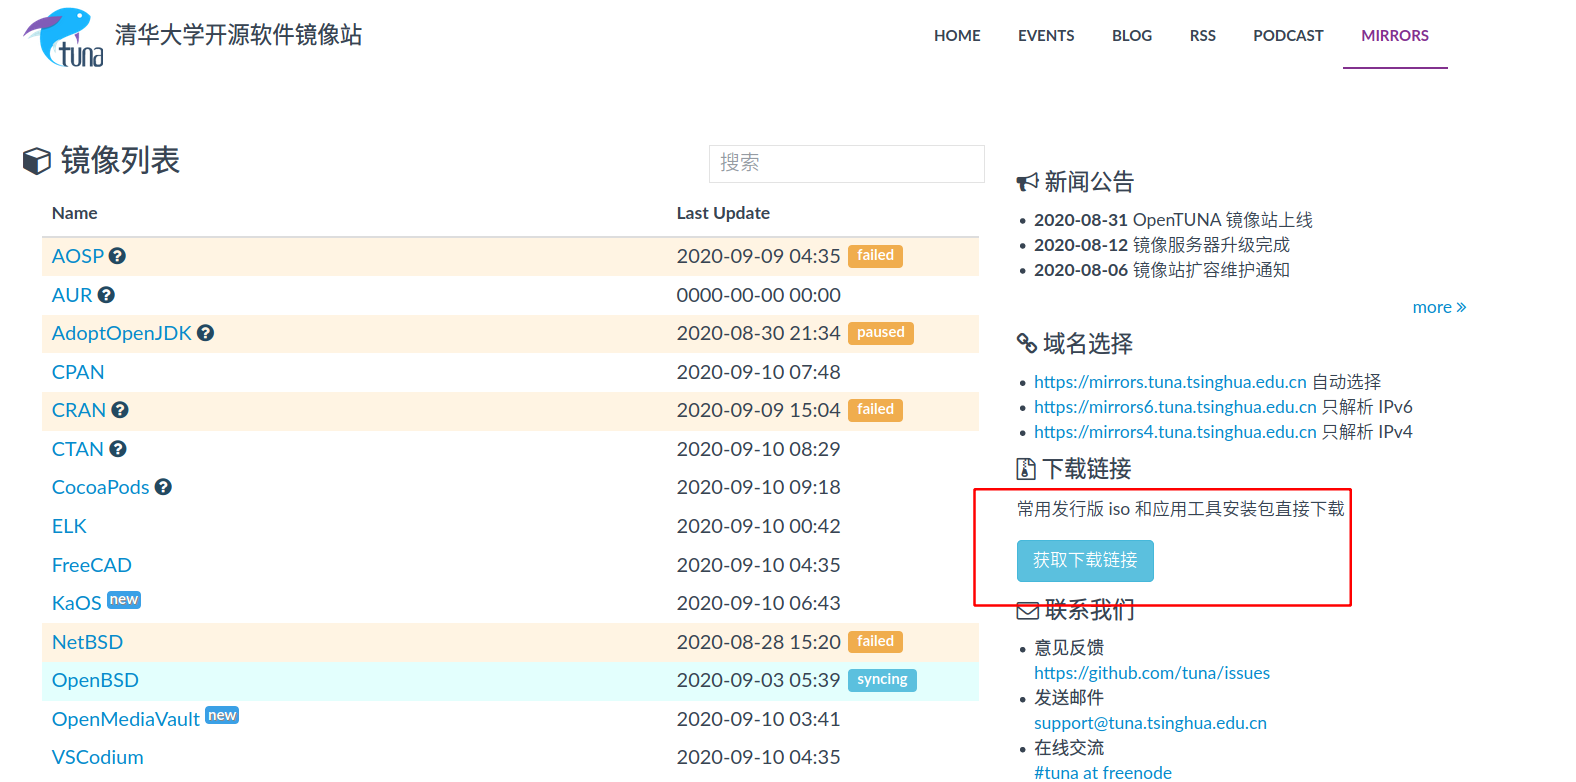
\includegraphics[width=0.6\linewidth]{./img/install/1.png}}\\
	\subfloat[2]{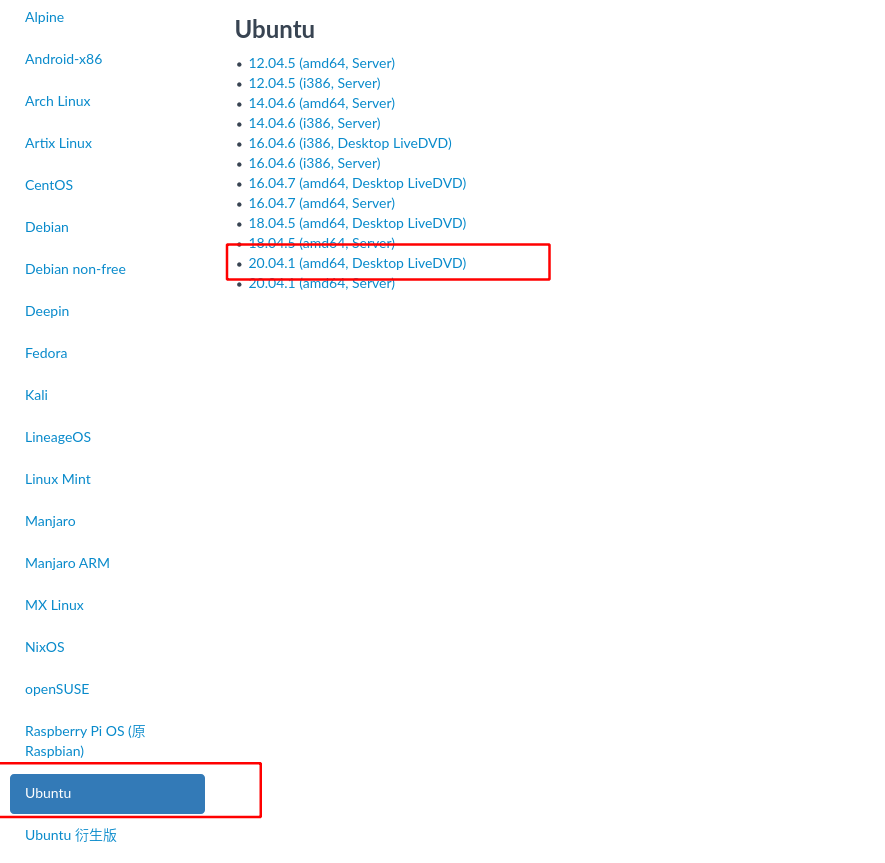
\includegraphics[width=0.6\linewidth]{./img/install/2.png}}
	\caption{镜像下载步骤}
\end{figure}

%\begin{verbatim}
%  https://mirrors.tuna.tsinghua.edu.cn/deepin-cd/
%\end{verbatim}
  
\section{制作启动盘镜像}
% window 系统下 
\flushleft
\begin{enumerate}
\item 如果在 window 系统下, 可以使用 Rufus, 选好镜像后,分区类型选GPT,刻录模式为DD

Rufus 下载地址:\\
\begin{lstlisting}
 https://share.weiyun.com/51nzNxs
\end{lstlisting}
\item 如果在 linux 系统下,可以使用 dd 命令。
\begin{lstlisting}

$ sudo fdisk -l 

# 我的U盘分区: /dev/sdc
$ umount /dev/sdc1
$ sudo mkfs.vfat /dev/sdc -I

# 我本地 ubuntu 镜像的完整路径:/home/gog/下载/ubuntu-20.04.1-desktop-amd64.iso 
# U盘分区: /dev/sdc
$ cd /home/gog/下载/
$ sudo dd bs=4M if=ubuntu-20.04.1-desktop-amd64.iso of=/dev/sdc status=progress
\end{lstlisting}

\section{分区建议}
这是一个建议的分区,而不是必须的,仅供参考, 这里以 250G 为例:


\begin{tabular}{|l|c|r|}
\hline
 挂载点 & 分区大小(G) & 占比(百分比)\\
\hline
   / & 100 & 40 \\      
\hline
   /home & 100 & 40 \\      
\hline
  交换分区(/swap) & 8 & \\
\hline
  efi分区(/boot/efi) & 0.2 & \\
\hline
  /boot & 0.2 & \\
\hline

\end{tabular}
\end{enumerate}


\setlength\parindent{2em}这里分区有几点要说明一下:

\begin{itemize}
\item 根分区和 home分区占大比重,其中 home 你可以在最后分,把剩下的所有的都给它。
\item 这里的换算: 1GB = 1000MB \footnote{在数学换算里 1G = 1024M,但是这里是 1000M}
\end{itemize}
